\section{Integrales}

\begin{multicols}{2}
Cuando se calcula la integral de una función se está averiguando su primitiva. El teorema fundamental del cálculo o teorema de Barrow dice que una integral definida es evaluar a la primitiva en los dos puntos y restarlas.

Recordar que se puede pensar la integral como sumar infinitos rectángulos entre la función y el eje $x$.
\vfill
\null

\begin{figure}[H]
    \centering
    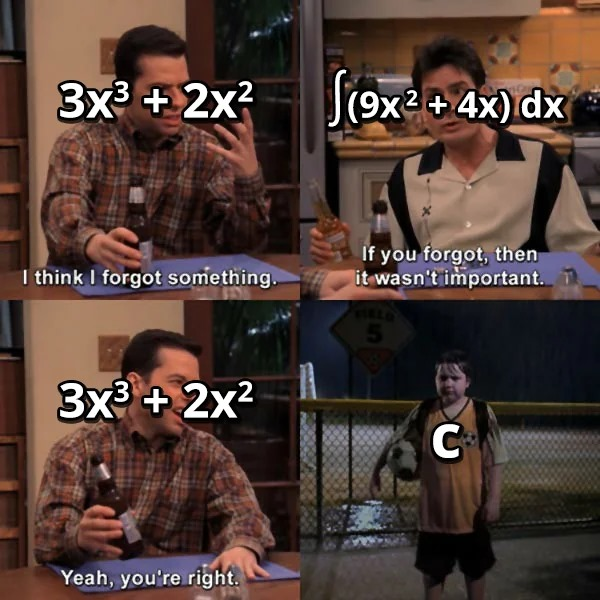
\includegraphics[width=0.9\linewidth]{Images/meme_integrales.jpg}
\end{figure}
\end{multicols}

\subsection*{Integración por sustitución}

Se basa en reemplazar una parte de la integral por una nueva variable $u$ y el resto por $du$. Es útil cuando se identifica que una parte es la derivada de otra parte. Para obtener $du$ se agarra lo que es igual a $u$, se lo deriva y se le agrega $dx$.
\skipline 

\underline{Ejemplo:}

\hfil
$\int \sin^2(x) \cdot \cos(x) \;dx\longrightarrow$
\begin{minipage}[c]{0.15\textwidth}
\begin{align*}
    u &= \sin(x)\\
    du &= \cos(x) \;dx
\end{align*}    
\end{minipage}
$\Longrightarrow \int u^2\;du = \dfrac{u^3}{3} + C= \dfrac{\sin^3(x)}{3} + C$
\hfil


\subsection*{Integración por partes}

Se basa en tener un producto de funciones dentro de la integral (\underline{u}n \underline{d}ía \underline{v}i \underline{u}na \underline{v}aca \underline{v}estida \underline{d}e \underline{u}niforme).

$$\int u \;dv = u\cdot v - \int v\;du$$

\skipline 

\underline{Ejemplo:}

\hfil
$\int x^2 \cdot \ln(x)\;dx \longrightarrow$
\begin{minipage}[c]{0.25\textwidth}
\begin{align*}
    u &= \ln(x) &&\;\;\;v= \dfrac{x^3}{3}\\
    du &= \dfrac{1}{x} \;dx &&\;dv = x^2 \;dx
\end{align*}    
\end{minipage}
$\;\;\Longrightarrow \ln(x) \cdot \dfrac{x^3}{3} \;- $ {\Large$\int$ }$ \dfrac{x^3}{3}\cdot \dfrac{1}{x}\;dx $
\hfil
\skipline

$$\Longrightarrow \ln(x)\cdot \dfrac{x^3}{3} - \dfrac{1}{3}\int x^2\;dx = \ln(x)\cdot \dfrac{x^3}{3} - \dfrac{1}{3} \cdot \dfrac{x^3}{3} + C=
\ln(x)\cdot \dfrac{x^3}{3} - \dfrac{x^3}{9} + C$$


\newpage
\subsection*{Teorema fundamental de cálculo}


\subsection*{Parte 1}

$$\Big(\int\limits^{u(x)}_a f(t)\;dt\Big)' = 
f\big(u(x)\big) \cdot u'(x)$$


\subsection*{Parte 2: Integrales definidas (Barrow)}

$$\int\limits^{b}_a f(x)\;dx = 
F(b)-F(a)$$

La integral definida de una función entre dos puntos es el área (con signo) entre la función y el eje $x$.

\vspace{\baselineskip}
\noindent
\underline{Ejemplo:}

$$\int\limits^{1}_{-3} x^2 + 1\;dx =
\dfrac{x^3}{3} + x\;\Bigg |^{1}_{-3} =
\dfrac{1^3}{3} + 1 - \left( \dfrac{(-3)^{3}}{3} + -3\right) =
\dfrac{4}{3} - (-12) = \dfrac{40}{3}
$$

Para calcular el área entre dos funciones, hacer la integral definida de techo menos piso, siendo los extremos de integración las intersecciones.

$$A = \int\limits_{a}^b f(x) - g(x) \;dx$$


\subsubsection*{Propiedades}

\begin{itemize}
    \item $\int\limits_a^c f(x)\,dx = \int\limits_a^b f(x)\,dx + \int\limits_b^c f(x) \,dx$
    
    \item $\int\limits^b_a f(x) \,dx=- \int\limits_b^a f(x)\,dx$
\end{itemize}


\subsection*{Integrales impropias}

Son integrales definidas donde el intervalo de integración tiene por extremo a algún infinito, a puntos que no están en el dominio o el intervalo de integración no es continuo.

Para solucionar los problemas, se hace lo siguiente:

$$\int\limits^\infty_a f(x)\;dx = \lim\limits_{b\rightarrow \infty} \int\limits^b_a f(x) \;dx = \lim\limits_{b\rightarrow \infty} F(b) - F(a)$$

Esto se tiene que hacer para cada singularidad. En caso que el límite exista y sea finito, se dice que la integral existe, caso contrario la integral no existe.

Un caso bastante común es el de $\int\limits_1^\infty x^n\;dx$. Esta integral diverge para valores $n\geq-1$.